\documentclass{article}
\usepackage{graphicx} %package to manage images
\usepackage[utf8]{inputenc}
\usepackage[a4paper, total={6in, 8in}]{geometry}
\usepackage{xurl}
\usepackage{hyperref}
\usepackage{float}

\title{Relatório 15 \\ Duração dos vídeos}
\author{Pedro A. S. O. Neto}
\date{Novembro, 2022}

\begin{document}

\maketitle

\section{Durações}

Foram analisados:

\begin{itemize}
  \item Tempo total de duração de cada vídeo, para cada participante
  \item Sample rate reportado pelo Tobii ($\Delta t$ entre linhas consecutivas do Computer.timestamp)
\end{itemize}

\section{Resultados}

As durações dos vídeos variam entre sujeito, e até mesmo entre diferentes aplicações para o mesmo sujeito. Na Figura 1, podemos visualiza a distribuição das durações dos vídeos. Os outliers com duração abaixo da mediana se devem ao fato de que alguns vídeos foram interrompidos durante o procedimento.

\begin{figure}[]
  \caption{Duração de cada vídeo, para cada participante}
  \noindent\makebox[\textwidth]{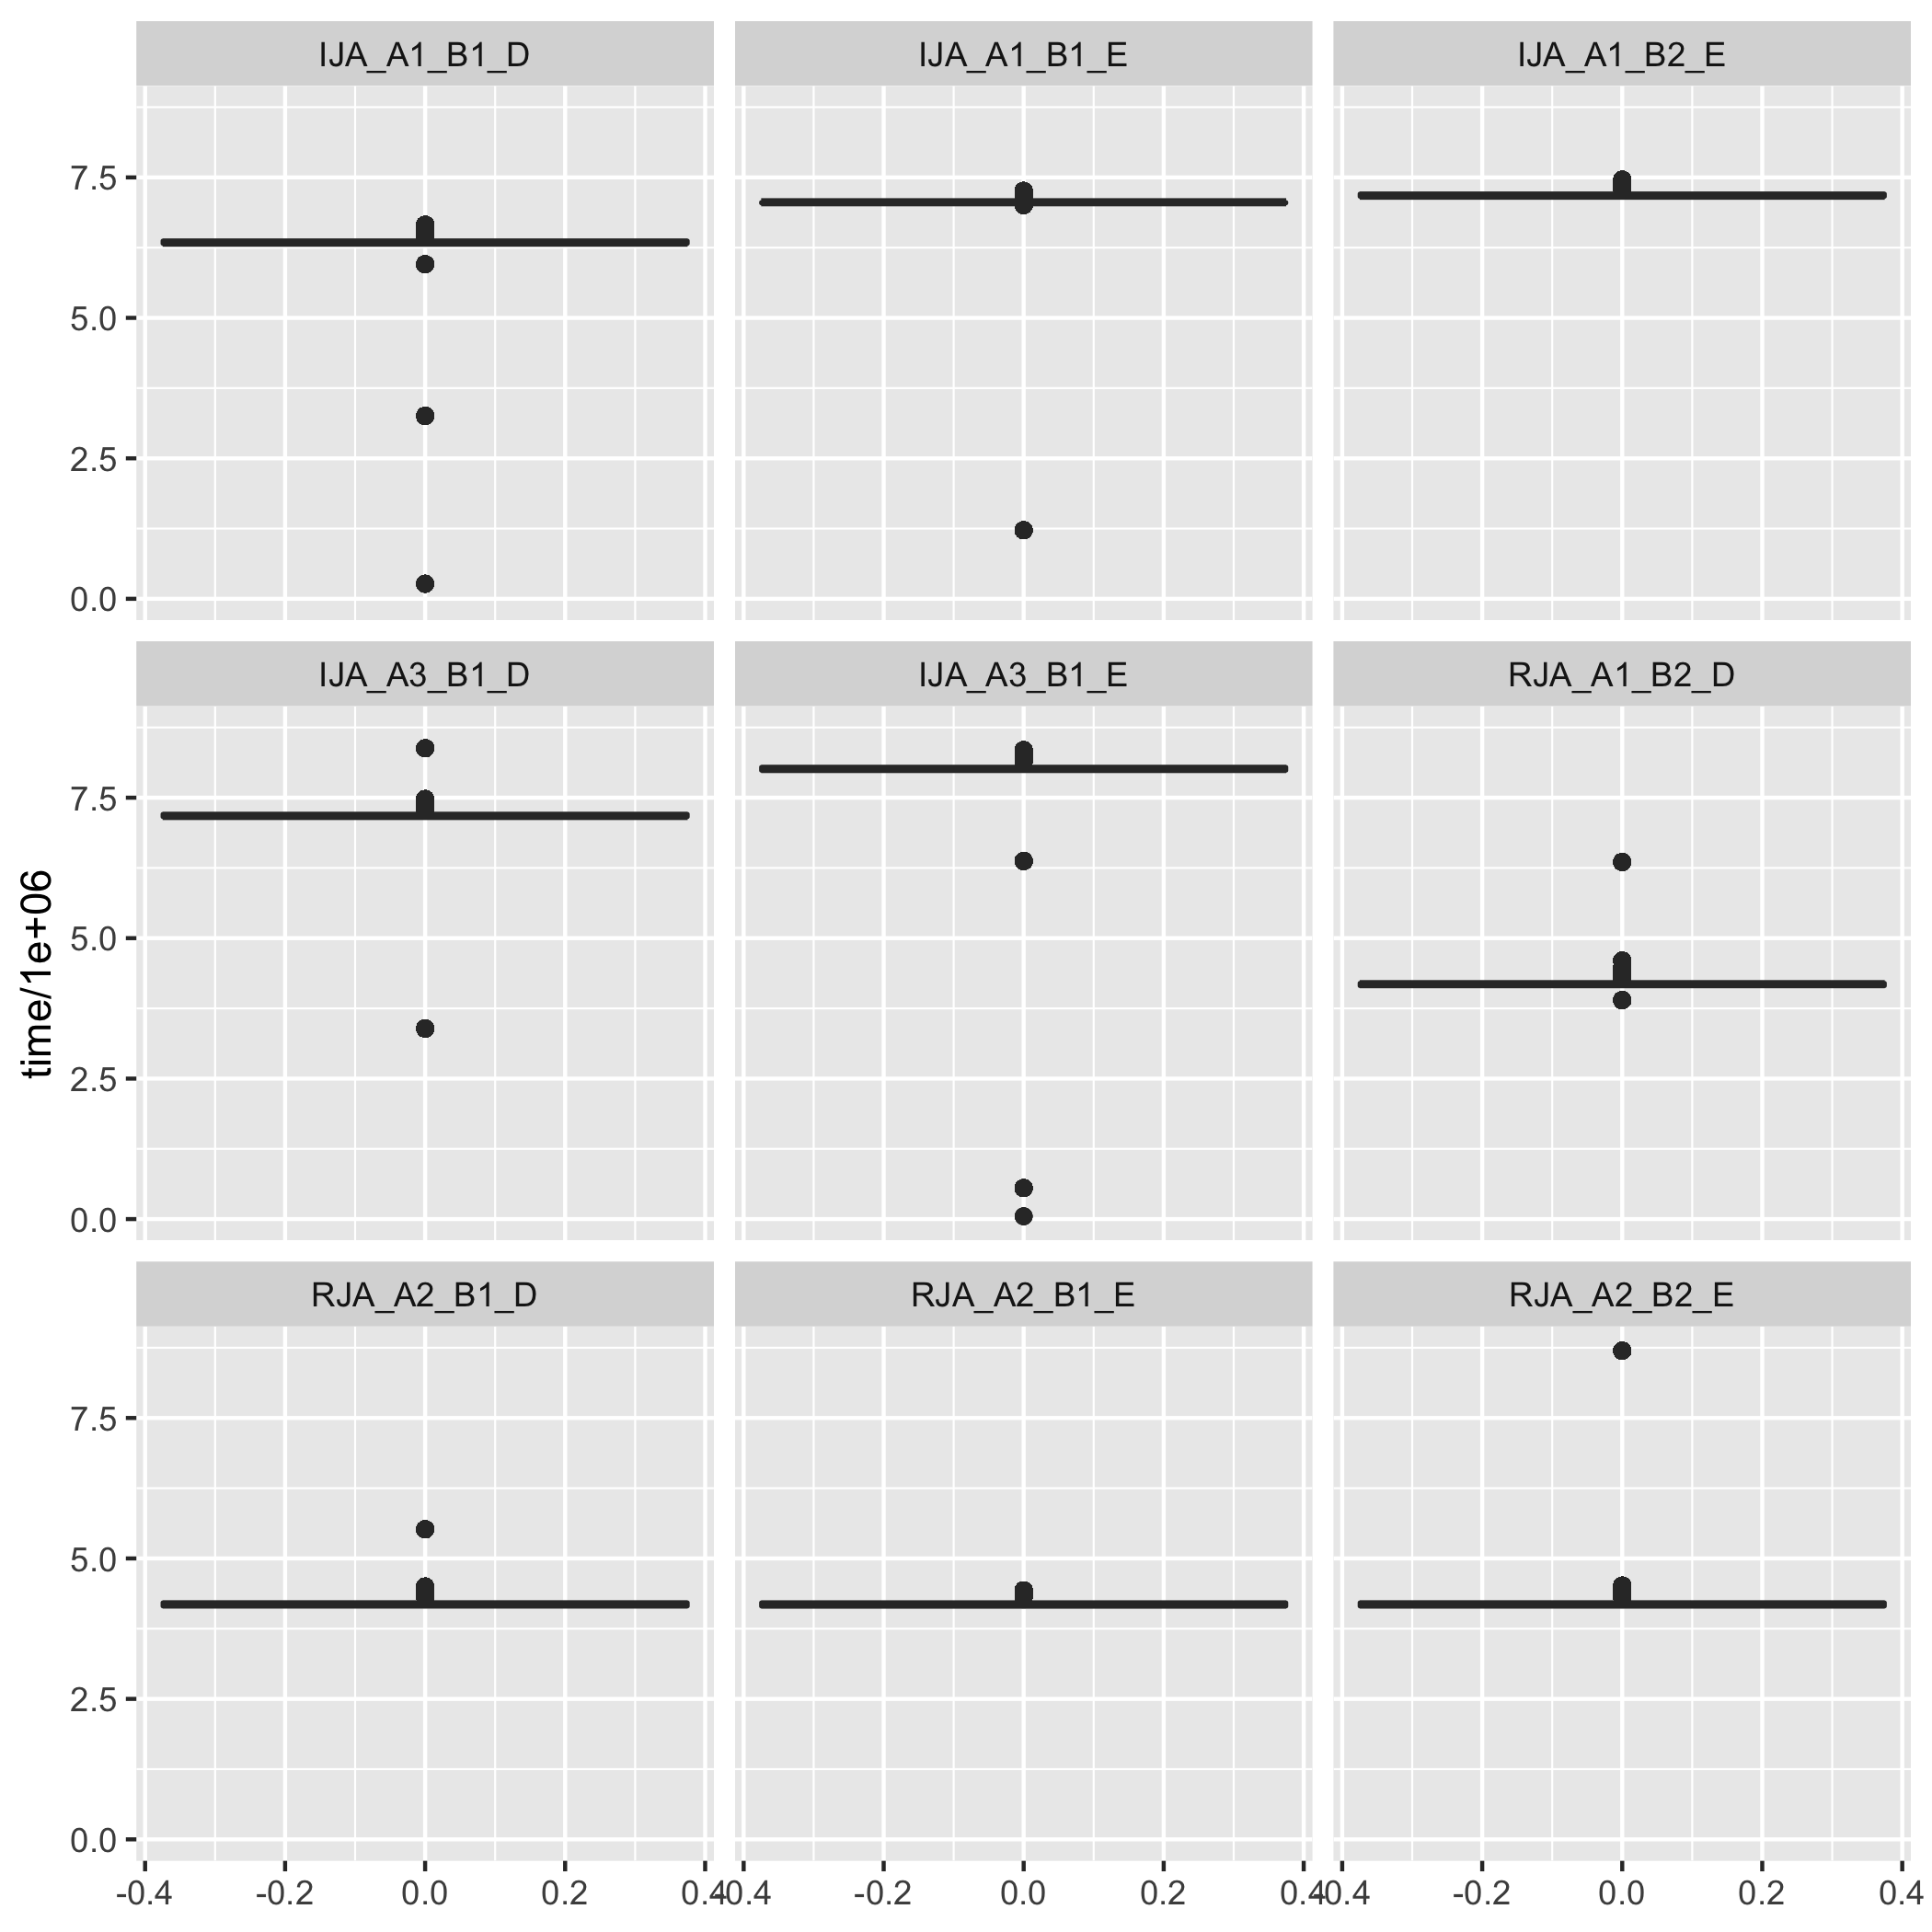
\includegraphics[scale=0.2]{./durations.png}}
  \centering
\end{figure}

\begin{figure}[]
  \caption{Duração do maior outlier identificado. O vídeo RJA\_A2\_B2\_E foi apresentado duas vezes para o participante CR641IP. Na primeira apresentação, o vídeo teve duração normal, porém negunda apresentação, a duração foi duas vezes maior do que a sua duração original}
  \noindent\makebox[\textwidth]{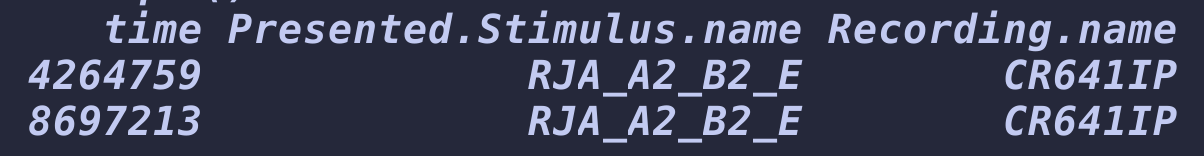
\includegraphics[scale=0.6]{./outlierExample.png}}
  \centering
\end{figure}

Uma possível explicação para durações anômalas de alguns vídeos seria algum problema na taxa de aquisição da Tobii. Nós investigamos, então, o $\Delta t$ entre linhas consecutivas no vídeo RJA\_A2\_B2\_E, do participante CR641IP (exemplo de outlier). No entanto, a taxa de aquisição não apresentou nenhuma inconsistência.

Os outliers acima da mediana não têm explicação, e ainda estamos investigando o que poderia causar, por exemplo, o vídeo RJA\_A2\_B2\_E do participante CR641IP ter uma duração 4 segundos superior à sua duração original. O Victor assistiu ao vídeo e notou que há, de fato, algo estranho na timeline desse participante. Mas ainda estamos em busca de uma possível causa.

\end{document}


